\documentclass[border=10pt]{standalone}
\usepackage{pgfplots}
\pgfplotsset{trig format plots=rad}
\begin{document}
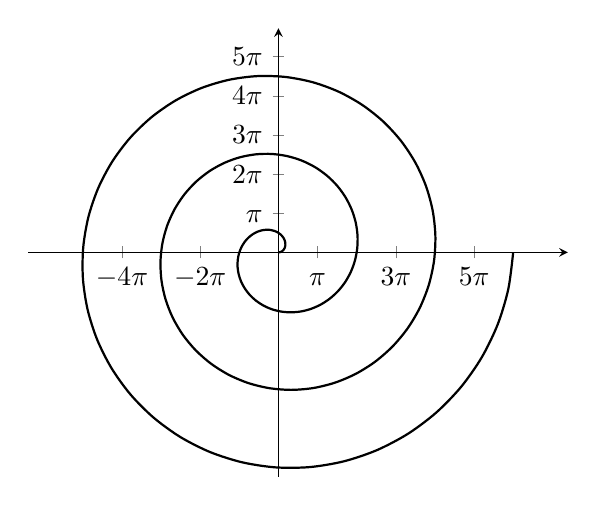
\begin{tikzpicture}
  \begin{axis}[axis lines = middle, axis equal,
      domain = 0:6*pi, ymin=-18, ymax=18,
      xtick = {-4*pi,-2*pi,pi,3*pi,5*pi},
      ytick = {pi, 2*pi, 3*pi, 4*pi, 5*pi},
      xticklabels = {$-4\pi$, $-2\pi$,
        $\vphantom{1}\pi$, $3\pi$, $5\pi$},
      yticklabels = {$\vphantom{1}\pi$, $2\pi$,
        $3\pi$, $4\pi$, $5\pi$}
    ]
    \addplot[samples=120, smooth, thick, variable=t]
      ( {t*cos(t)}, {t*sin(t)} );
  \end{axis}
\end{tikzpicture}
\end{document}
